\documentclass[usletter]{article}
\usepackage{amsthm}
\usepackage{mathtools}
\usepackage{multicol}

\usepackage{hw}
\usepackage[margin=1.5in]{geometry}
\usepackage{comment}
\usepackage{url}
\usepackage{enumitem}

\usepackage{tikz}
\usetikzlibrary{automata, positioning}
\usetikzlibrary{arrows}

\begin{document}

\makeheader{First \& Last Name}	% your name
           {100-200-300}          		% your university id
           {01}                     			% unused
           {Automata and Languages}	% lecture title

\noindent

\begin{itemize}
\item Grade: 100\% = Problem \ref{p1} ($40\%$) + Problem \ref{p2} ($30\%$) + Problem \ref{p3} ($30\%$)
\item Homework 1 is due no later than Thursday 07/14/2016 23:55 as a file on \url{ccle.ucla.edu}, or submitted at the discussion section on a paper
\item Homework file can be in \LaTeX\ (template to be given) or Microsoft Word
\item Have a question? \url{piazza.com/ucla/summer2016/cs181}
\end{itemize}

%\newpage

\bigskip
\begin{problem}
\label{p1}
Are the following equalities correct or not? Prove your answers ($20$ pts/question)

%\medskip

For all sets $A$, $B$, and $C$:
\begin{enumerate}[label=(\alph*)]
\item $A \cap (B \cup C) = (A \cap B) \cup (A \cap C)$
\item $A {\ \backslash\ } (B \cup C) = (A {\ \backslash\ } B) \cup (A {\ \backslash\ } C)$
\end{enumerate}
\end{problem}

\begin{answer}for Problem \ref{p1}:
%Solution goes here.
\end{answer}


\medskip
%-------------------------------------------------------------------------------
\begin{problem}
\label{p2}

Draw a DFA and an NFA recognizing the following language in the binary alphabet $\big\{0,1\big\}$

$\big\{ w | w \text{ contains an even number of }0\text{s, or contains exactly two }1\text{s}\big\}$
\end{problem}

\begin{answer}for Problem \ref{p2}:
%Solution goes here.
\end{answer}

\medskip
%-------------------------------------------------------------------------------
\begin{problem}
\label{p3}
Convert the following automaton into the equivalent DFA:


\begin{center}
	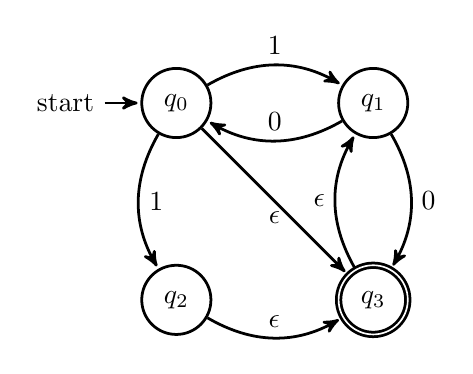
\begin{tikzpicture}[node distance=25mm, auto, line width=1pt, ->,>=stealth',shorten >=1pt]
	\node[state,initial]   (sq1)                      {$q_0$};
	\node[state         ]   (sq2) [right of=sq1]  {$q_1$};
	\node[state         ]   (sq3) [below of=sq1]  {$q_2$};
	\node[state,accepting]   (sq4) [right of=sq3]  {$q_3$};
	
	\path[->, line width=1pt, ->,>=stealth',shorten >=1pt]
			(sq1) edge[bend left]  node {$1$} (sq2)
			(sq2) edge[bend left,above]  node {$0$} (sq1)
			(sq2) edge[bend left]  node {$0$} (sq4)
			(sq4) edge[bend left]  node {$\epsilon$} (sq2)
			(sq1) edge[bend right]  node {$1$} (sq3)
			(sq1) edge[below] node {$\epsilon$} (sq4)
			(sq3) edge[bend right]  node {$\epsilon$} (sq4);
	\end{tikzpicture}
\end{center}

\end{problem}

\begin{answer}for Problem \ref{p3}:
%Solution goes here.
\end{answer}
%-------------------------------------------------------------------------------


\bibliographystyle{abbrv}
\bibliography{template}

\end{document}
